% IF YOU ARE USING OVERLEAF, MAKE SURE TO SET THE COMPILER TO XeLatex.

\documentclass[final]{beamer}

% ====================
% Packages
% ====================

\usepackage[T1]{fontenc}
\usepackage{lmodern}
\usepackage[size=custom,width=91.44,height=60.96,scale=0.83]{beamerposter}
\usetheme{gemini}
\usecolortheme{stanford}
\usepackage{graphicx}
\usepackage{booktabs}
\usepackage{tikz}
\usetikzlibrary{shapes,arrows,positioning,calc}
\usepackage{pgfplots}
\usepackage{amsmath}
\usepackage{amssymb}
\usepackage{siunitx}
\pgfplotsset{compat=1.17}
\graphicspath{{figures/project/}{stanford_logos/}}

% Tighten vertical spacing between poster blocks.
\addtobeamertemplate{block end}{}{\vspace{-0.45cm}}

% ====================
% Lengths
% ====================

\newlength{\sepwidth}
\newlength{\colwidth}
\setlength{\sepwidth}{0.01\paperwidth}
\setlength{\colwidth}{0.32\paperwidth}
\newcommand{\separatorcolumn}{\begin{column}{\sepwidth}\end{column}}

% ====================
% Title
% ====================

\title{Decision Transformer Warm-Start for Minimum-Time Vehicle Trajectory Optimization}
\author{Sebastian Martinez}
\institute[shortinst]{Department of Aeronautics \& Astronautics, Stanford University}

\footercontent{
  \href{mailto:sebasmp@stanford.edu}{sebasmp@stanford.edu} \hfill
  Stanford CS234: Reinforcement Learning \hfill
  Decision Transformer Warm-Starts for Trajectory Optimization
}

\begin{document}

\addtobeamertemplate{headline}{}
{
    \begin{tikzpicture}[remember picture,overlay]
      \node [anchor=north east, inner sep=3cm] at ([xshift=1.0cm,yshift=2.5cm]current page.north east)
      {
\includegraphics[height=6.0cm]{Block_S_2_color.png}};
    \end{tikzpicture}
}

\begin{frame}[t]
\begin{columns}[t]
\separatorcolumn

\begin{column}{\colwidth}

\begin{block}{Problem}
Minimum-time racing line optimization is a drive-at-the-limits planning problem in which lateral and longitudinal forces must be coordinated near the tire friction boundary while satisfying strict track and safety constraints. In this regime, trajectory quality and solver behavior depend strongly on the fidelity of the vehicle model used in the nonlinear program [1].

The objective is to determine whether an offline sequence model can amortize this nonlinear constrained optimization problem by supplying a better warm start. The target setting is closed-track autonomous racing with nonlinear vehicle dynamics, hard track boundaries, and static obstacle-avoidance constraints.

The system is two-stage: a planner based on spatial direct collocation and a single-track vehicle model generates expert trajectories, while a Decision Transformer (DT) learns from this offline data to predict warm-start trajectories $(X_{\text{init}}, U_{\text{init}})$. The goal is to reduce solver iterations and wall-clock solve time without sacrificing feasibility or lap time quality.

This hybrid framing keeps hard dynamics and safety constraints inside the optimizer while shifting part of the repeated search effort into an offline-trained sequence model.
\end{block}

\begin{block}{Background}
The planner is a \textbf{minimum-time nonlinear program} in Frenet coordinates solved by \textbf{spatial direct collocation}. It uses a nonlinear single-track vehicle model configured to the 2018 VW Golf GTI test vehicle from prior Stanford autonomous-racing work [1]. The optimizer minimizes lap time while enforcing dynamics, track bounds, forward progress, and obstacle-clearance constraints, and its accepted solutions also provide the expert trajectories used for learning.
\begin{align*}
 \min_{x_{0:N},\,u_{0:N}} \quad & t_N \;+\; \lambda_u\sum_{k=0}^{N-1}\lVert u_{k+1}-u_k\rVert^2 \\[4pt]
\text{s.t.} \quad
& x_{k+1} = x_k + \frac{\Delta s}{2}\Big(f_s(x_k,u_k)+f_s(x_{k+1},u_{k+1})\Big), \quad k=0,\dots,N-1 \\
& e_{\min}(s_k)\le e_k\le e_{\max}(s_k),\quad |\delta_k|\le\delta_{\max},\quad F_{x,\min}\le F_{x,k}\le F_{x,\max} \\
& \dot{s}_k \ge \epsilon_s,\quad 1-\kappa(s_k)e_k \ge \epsilon_\kappa \\
& \lVert p(s_k,e_k)-p_{\mathrm{obs},i}\rVert^2 \ge R_{\mathrm{safe},i}^2
\end{align*}

For the learning component, \textbf{Decision Transformer} is used as an offline RL method based on conditional sequence modeling [2]. The model is trained on optimizer-generated trajectories and conditioned on return-to-go, state, and action history. The approach is inspired by \textbf{ART} (Autonomous Rendezvous Transformer), which applies the same learned warm-start idea to spacecraft rendezvous trajectory optimization [3]. In this setting, the DT is not the final controller: it proposes a warm start for the downstream optimizer.
\end{block}

\begin{block}{Methods}
    \vspace{-5pt}

\begin{figure}
\centering
\begin{tikzpicture}[
    node distance=1cm,
    layer/.style={rectangle, draw, rounded corners, minimum height=0.95cm, text width=8.8cm, align=center, font=\small, very thick},
    token/.style={font=\scriptsize},
    arrow/.style={->, >=stealth, thick}
]
\node[layer, fill=red!10] (opt) {Constrained optimization: FATROP};
\node[layer, fill=gray!12, below=of opt] (dyn) {Dynamics rollout};
\node[layer, fill=blue!18, below=of dyn] (dt) {Decision Transformer warm-start model};

\node[token, below=0.2cm of dt.south west, anchor=north east] (rtg) {$R(t_i)$};
\node[token, right=0.5cm of rtg] (ctx) {track / obstacle context};
\node[token, right=0.62cm of ctx] (state) {$x(t_i)$};
\node[token, right=0.62cm of state] (act) {$u(t_i)$};
\draw[arrow] (rtg.north) -- (dt.south west);
\draw[arrow] (ctx.north) -- ($(dt.south west)!0.33!(dt.south east)$);
\draw[arrow] (state.north) -- ($(dt.south west)!0.58!(dt.south east)$);
\draw[arrow] (act.north) -- ($(dt.south west)!0.80!(dt.south east)$);

\draw[arrow] ($(dt.north)+(0,0.0)$) -- node[right, font=\scriptsize] {$\hat{u}(t_i), \hat{u}(t_{i+1}), \dots$} (dyn.south);
\draw[arrow] ($(dyn.north)+(0,0.0)$) -- node[right, font=\scriptsize, align=center] {accepted warm start} (opt.south);
\draw[arrow] ($(opt.north)+(0,0.0)$) -- ++(0,0.55) node[right, font=\scriptsize] {feasible minimum-time trajectory};

\node[token, left=0.5cm of dt.west, align=right] {offline\\expert data};
\draw[arrow] ([xshift=-0.55cm]dt.west) -- ([xshift=-0.02cm]dt.west);
\end{tikzpicture}
\caption{Offline warm-start pipeline.}
\end{figure}

% \vspace{0.4em}
%
% \begin{center}
% \begin{tikzpicture}[
%     node distance=0.5cm,
%     tok/.style={rectangle, draw, rounded corners, minimum height=0.8cm, text width=1.55cm, align=center, font=\scriptsize},
%     proc/.style={rectangle, draw, rounded corners, minimum height=0.95cm, text width=2.45cm, align=center, font=\scriptsize},
%     arrow/.style={->, >=stealth, thick}
% ]
% \node[tok, fill=blue!14] (rtgk) {$R_k$};
% \node[tok, fill=blue!14, right=of rtgk] (xk) {$\tilde{x}_k$};
% \node[tok, fill=blue!14, right=of xk] (uk) {$u_k$};
% \node[tok, fill=blue!14, right=of uk] (rtgkp) {$R_{k+1}$};
% \node[tok, fill=blue!14, right=of rtgkp] (xkp) {$\tilde{x}_{k+1}$};
% \node[tok, fill=blue!14, right=of xkp] (ukp) {$u_{k+1}$};
% \node[proc, fill=green!14, right=0.75cm of ukp] (embed) {Embeddings};
% \node[proc, fill=orange!18, right=of embed] (trans) {Causal DT\\$K=50$, 6L, 4H, 192D};
% \node[proc, fill=gray!18, right=of trans] (head) {Predict $\hat{u}_k$\\and $\hat{x}_{k+1}$};
%
% \draw[arrow] (rtgk) -- (xk);
% \draw[arrow] (xk) -- (uk);
% \draw[arrow] (uk) -- (rtgkp);
% \draw[arrow] (rtgkp) -- (xkp);
% \draw[arrow] (xkp) -- (ukp);
% \draw[arrow] (ukp) -- (embed);
% \draw[arrow] (embed) -- (trans);
% \draw[arrow] (trans) -- (head);
% \end{tikzpicture}
% \end{center}
%
% \begin{center}
% \scriptsize\textit{Figure 2. Decision Transformer tokenization and prediction flow.}
% \end{center}
\end{block}

\end{column}

\separatorcolumn

\begin{column}{\colwidth}
    \vspace{30pt}

\noindent The method combines offline trajectory optimization, sequence-model training, and solver warm-starting. As shown in Figure 1, the nonlinear optimizer first generates accepted expert trajectories offline. These trajectories are then converted into training sequences for a \textbf{Decision Transformer}, so the learning problem is treated as \textbf{offline RL via sequence modeling} rather than online policy search. Each tokenized sequence contains return-to-go, augmented state, and action history. The augmented state includes the local vehicle/path state $(u_x,u_y,r,e,\Delta\psi)$ together with track geometry and padded obstacle context. Return-to-go is computed from negative time increments, so larger return corresponds to less remaining lap time.

The DT is a causal transformer with context length $K=50$, $6$ layers, $4$ attention heads, embedding dimension $192$, batch size $128$, and dropout $0.1$. Training uses a supervised objective with action prediction plus an auxiliary next-state loss,
\[
 \mathcal{L}_k = \|u_k-\hat{u}_k\|_2^2 + \lambda_x \|x_{k+1}^{\mathrm{obs}}-\hat{x}_{k+1}^{\mathrm{obs}}\|_2^2,
\]
with the total loss averaged over valid sequence tokens and the latest improved parent run using $\lambda_x=0.1$. At inference, the model autoregressively predicts actions and rolls them forward through the vehicle dynamics to produce a candidate warm-start trajectory.

The downstream solver remains the same constrained minimum-time NLP used for expert generation. In the active pipeline, \textbf{FATROP} is used to generate clean expert trajectories and repair segments and to solve the downstream warm-started optimization problem. The DT therefore does not replace the optimizer: it provides an initialization that is refined and passed into the same solver stack.

\begin{block}{Experiments}
Experiments are conducted on an \textbf{Oval-first benchmark} with two fixed evaluation sets: a no-obstacle evaluation set and an obstacle evaluation set containing 1--4 circular obstacles. In each case, the DT generates a candidate warm-start trajectory for the same downstream FATROP minimum-time solver used to produce the expert data.

The offline dataset is built from multiple classes of optimizer-generated trajectories. The largest component is a shift dataset of accepted full-lap solutions circularly shifted along the track. This base distribution is augmented with targeted repair data intended to expose the model to more difficult rollout states: 400 hard repairs, 1{,}000 post-projection repairs, and 300 failure-conditioned repairs, in addition to 31{,}710 shift episodes.

Model inputs consist of return-to-go, local vehicle/path state, track features, and nearest-obstacle context, and the output is a warm-start control sequence together with the rolled-out state trajectory. Evaluation focuses on the downstream optimizer: the main metrics are warm-start acceptance, fallback behavior, solver iterations, and total solve time.
\begin{figure}
  \centering
  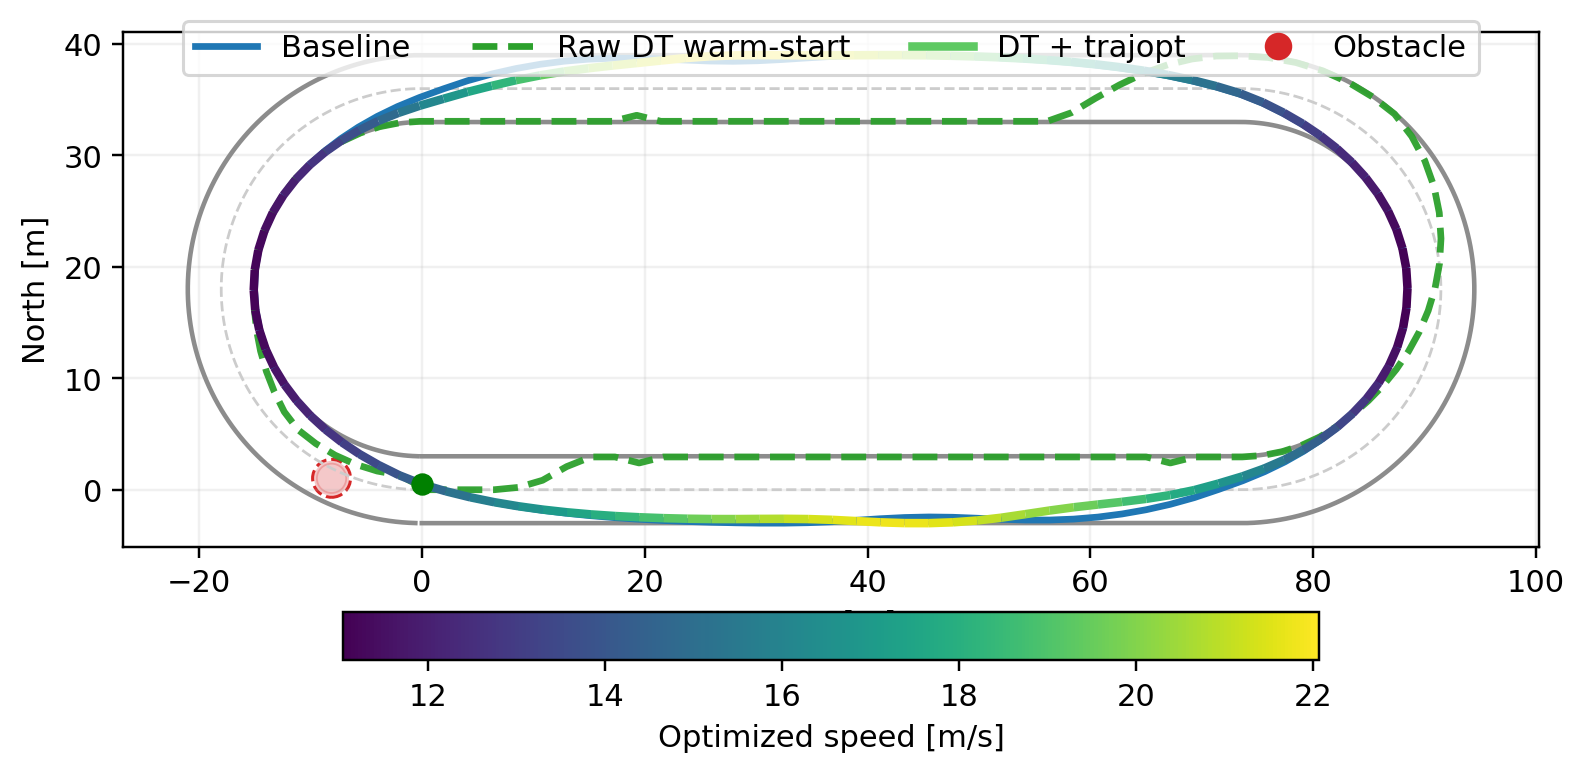
\includegraphics[width=0.92\linewidth]{scenario000_obs3_compare.png}
  \caption{Obstacle case from the corrected evaluation pipeline. The plot shows the baseline solution, the raw DT pre-solve warm-start, and the final optimized trajectory.}
\end{figure}
\end{block}

\end{column}

\separatorcolumn

\begin{column}{\colwidth}

\begin{figure}
  \centering
  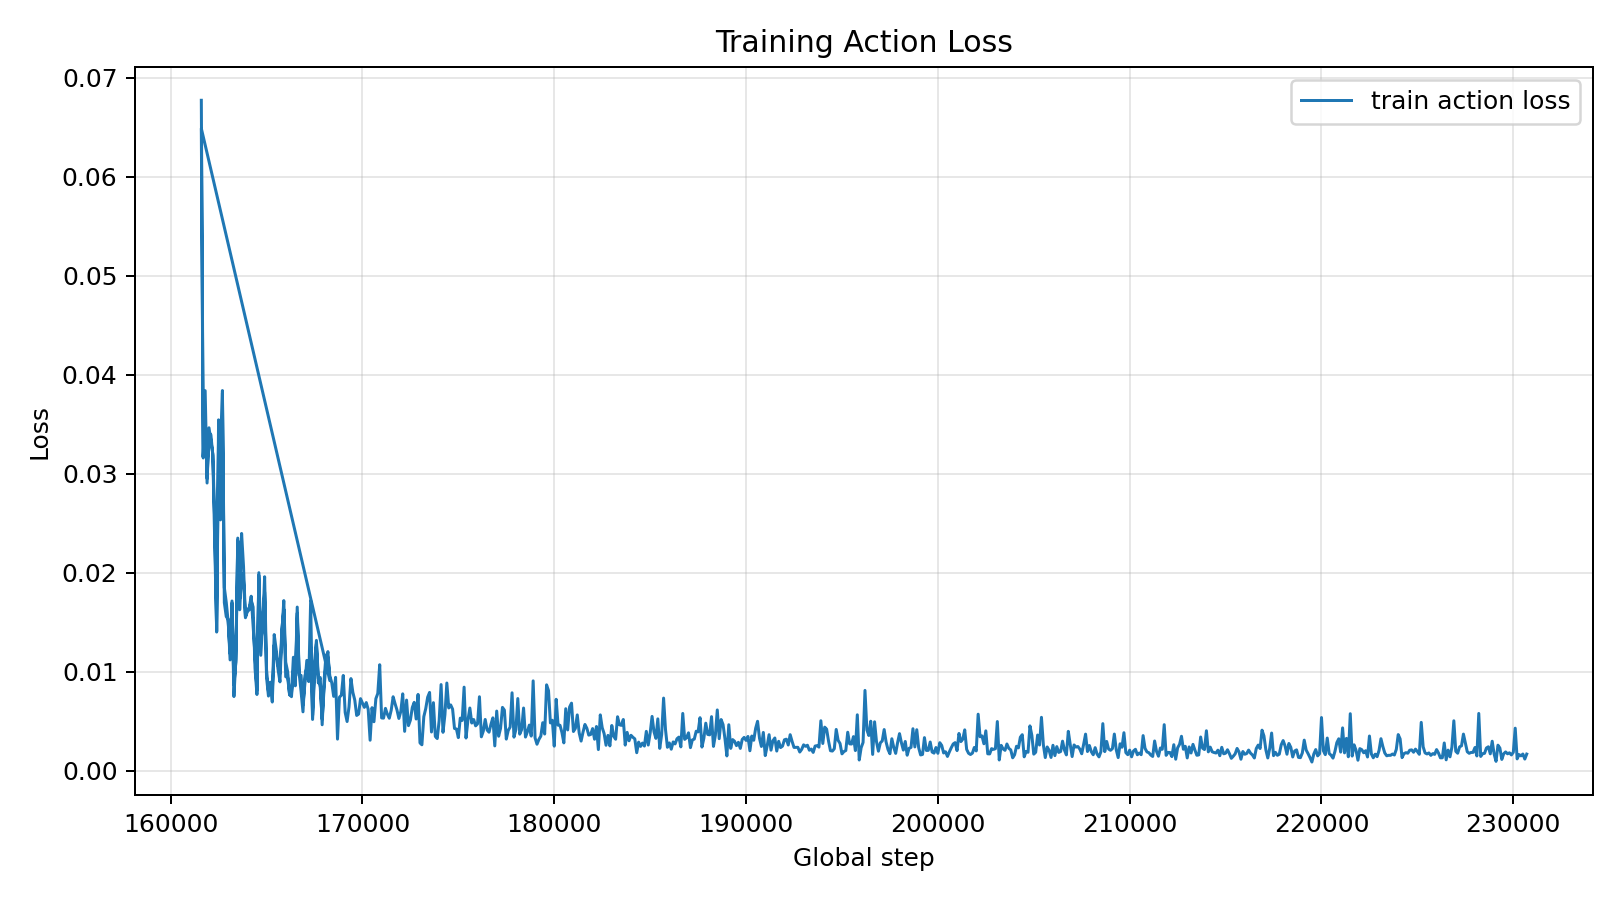
\includegraphics[width=0.58\linewidth]{postproj_ft2_train_loss_curves.png}
  \caption{Later fine-tuning runs trained stably under the larger-context DT setup.}
\end{figure}

\begin{block}{Results and Interpretation}
The project started from a parent DT trained on nominal Oval trajectories and then improved the warm-start pipeline through targeted training and debugging steps. In the later runs, the raw DT trajectories became more structured, handled obstacles more plausibly, and in some cases slightly reduced solver-only time. This showed that the DT was learning useful trajectory structure, even though the full warm-start pipeline was not yet consistently faster end to end.
\begin{itemize}
\item larger-context DT training improved nominal trajectory quality,
\item repair datasets exposed the model to harder rollout states,
\item rollout and evaluation fixes made downstream behavior much easier to interpret.
\end{itemize}
The table below shows the clearest evaluation setting after those improvements.
\begin{center}
\footnotesize
\setlength{\tabcolsep}{5pt}
\resizebox{\linewidth}{!}{%
\begin{tabular}{p{4cm}c c c p{8cm}}
\toprule
\textbf{Setting} & \textbf{WS accept} & \textbf{Baseline solve} & \textbf{DT total} & \textbf{Takeaway} \\
\midrule
No obstacles & `20\%` & `49.06s` & `51.98s` & raw DT trajectories were often reasonable, but total time did not improve yet \\
1--4 obstacles & `20\%` & `56.36s` & `60.79s` & obstacle-aware warm-starts were generated, but consistency still needs work \\
\bottomrule
\end{tabular}%
}
\end{center}

Across stricter evaluation settings, the same pattern remained: the DT could generate plausible warm-start trajectories, but not yet reliably enough to produce robust end-to-end gains.
\end{block}

\begin{block}{Conclusions and Next Steps}
The main contribution of the project is a working framework for learned warm-starts in constrained racing trajectory optimization. It combines offline training, repair-data generation, rollout diagnostics, and downstream benchmarking in one pipeline.

The most important result is that the DT learned meaningful trajectory structure and produced real warm-start signal, but deployment metrics remained much harder than offline training metrics. This made it clear that model selection in this setting has to be driven by acceptance, iterations, and total solve time, not training loss alone.

The next step is narrow: keep training on the difficult rollout states identified by the diagnostics so that the improved raw DT trajectory quality turns into more consistent optimizer gains.
\end{block}

\begin{block}{References}
\vspace{-12pt}
\footnotesize
\begin{enumerate}
  \item J. K. Subosits and J. C. Gerdes, ``Impacts of Model Fidelity on Trajectory Optimization for Autonomous Vehicles in Extreme Maneuvers,'' \textit{IEEE Transactions on Intelligent Vehicles}, 2021.
  \item L. Chen et al., ``Decision Transformer: Reinforcement Learning via Sequence Modeling,'' \textit{Advances in Neural Information Processing Systems}, 2021.
  \item T. Guffanti and S. D'Amico, ``Transformers for Trajectory Optimization with Application to Spacecraft Rendezvous,'' \textit{IEEE Aerospace Conference}, 2024.
\end{enumerate}
\end{block}

\end{column}

\separatorcolumn
\end{columns}
\end{frame}

\end{document}
